\documentclass[../main.tex]{subfiles}

\begin{document}
Para poder empezar con el modelado en Protegé se ha considerado como clases todas las características dentro del documento llamado \textbf{medicamentos.xlsx } tal y como se muestra en la siguiente imagen: \\

\begin{figure}[h]
    \centering
    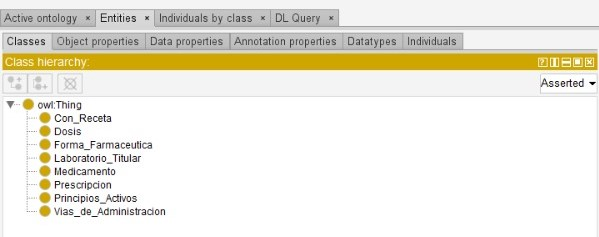
\includegraphics[scale=0.7]{images/protege-Clases.jpeg}
    \caption{Clases}
    \label{fig:mesh1}
\end{figure}


\vspace{2cm}
Se han creado además cuatro propiedades de tipo objeto que son: como adquirirlo que tiene como dominio la clase \textbf{Vías de Administración}, principio activo que tiene como dominio la clase \textbf{Principio Activo}, tipo de prescripción tien como dominio la clase \textbf{Prescripcion} y tipo de laboratorio tiene como dominio la clase de \textbf{Laboratorio Titular}.\\

\begin{figure}[h]
    \centering
    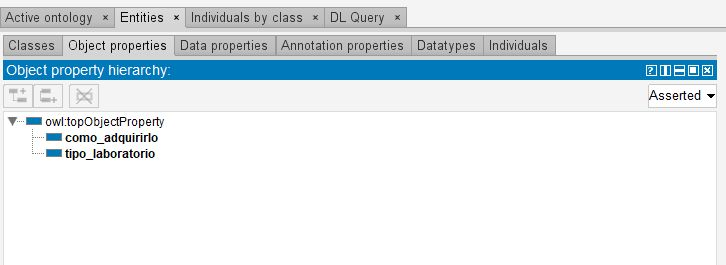
\includegraphics[scale=0.7]{images/protege-ObjectProperties.jpeg}
    \caption{Object Properties}
    \label{fig:mesh1}
\end{figure}

\vspace{1cm}
También, se han creado como propiedades de datos las tres siguientes: cantidad de dosis que se relaciona con la clase \textbf{Dosis}, como adquirirlo que se relaciona con la clase \textbf{Con Recetas} y tipo de forma farmacéutica que se relaciona con la clase \textbf{Forma Farmacéutica} Todas estas propiedades se han considerado de tipo \textit{string}. \\

\begin{figure}[h]
    \centering
    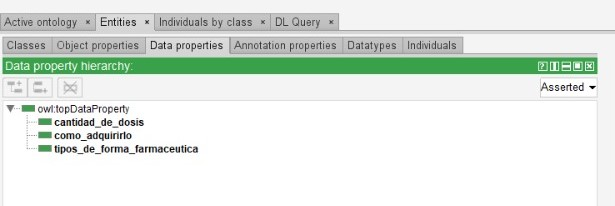
\includegraphics[scale=0.7]{images/protege-DataProperties.jpeg}
    \caption{Data Properties}
    \label{fig:mesh1}
\end{figure}

\vspace{2cm}
Se han creado varios tipos de principios activos, de laboratorios, de vías de administración y de tipos de prescripción para así poder crear de manera adecuada los cinco ejemplos de medicamentos para poder después trabajar con las queries en SPARQL.\\

\begin{figure}[h]
    \centering
    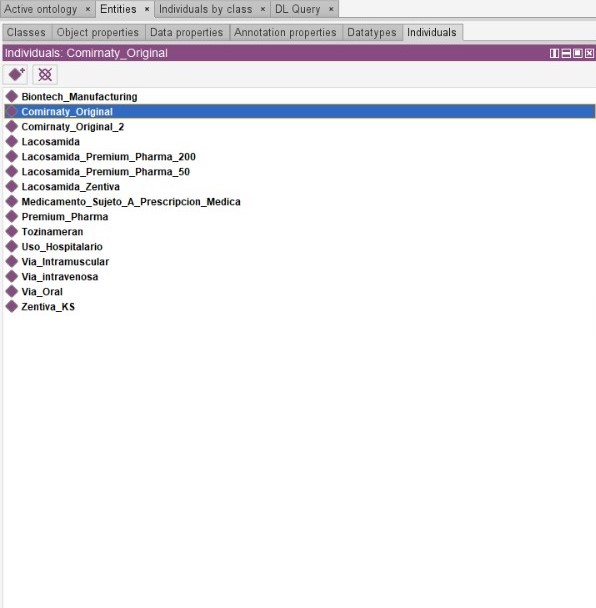
\includegraphics[scale=0.7]{images/protege-Individuals-pt1.jpeg}
    \caption{Individuals}
    \label{fig:mesh1}
\end{figure}

\begin{figure}[h]
    \centering
    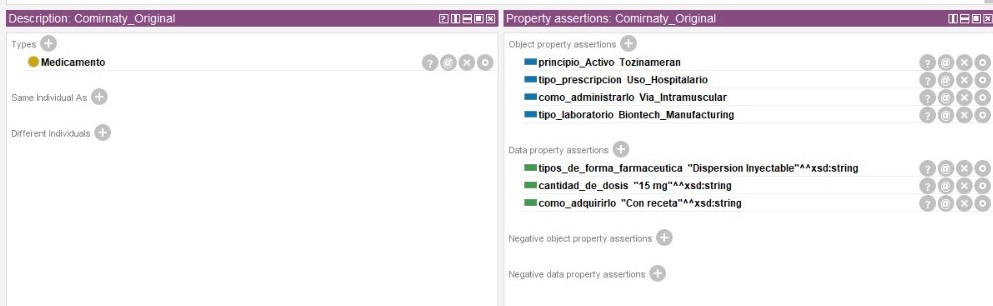
\includegraphics[scale=0.5]{images/protege-Individuals-pt2.jpeg}
    \caption{Individuals}
    \label{fig:mesh1}
\end{figure}

\vspace{1cm}
Finalmente, se ha generado un grafo con las clases que componen el modelado y los correspondientes ejemplos de individuals que hemos creado àra poder relacionar las clases: \\

\begin{figure}[h]
    \centering
    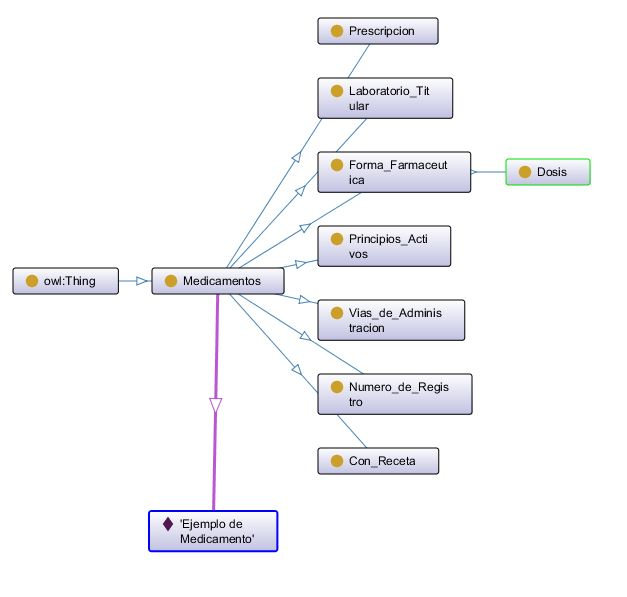
\includegraphics[scale=0.4]{images/protege-Grafo.jpeg}   \caption{Grafo}
    \label{fig:mesh1}
\end{figure}


\end{document}